\RequirePackage[l2tabu, orthodox]{nag} % Do not remove!

\documentclass[letterpaper, 10 pt, conference]{ieeeconf} % Comment this line out
                                                          % if you need a4paper
%\documentclass[a4paper, 10pt, conference]{ieeeconf}      % Use this line for a4
                                                          % paper

\IEEEoverridecommandlockouts                              % This command is only
                                                          % needed if you want to
                                                          % use the \thanks command
\overrideIEEEmargins
% See the \addtolength command later in the file to balance the column lengths
% on the last page of the document


%---------- Additional packages ----------
\usepackage{microtype}
\usepackage[all, nodollardollar]{onlyamsmath} % Do not remove!
\usepackage{mathtools}
\usepackage{fullpage}
\usepackage{hyperref}
\usepackage{comment}
\usepackage{setspace}
\usepackage{amsmath}
\usepackage{amssymb}
%\usepackage{amsthm}
\usepackage{etoolbox}
\usepackage{color,colortbl}
\usepackage{mathtools}
\usepackage{enumerate}
% \usepackage{algorithm, algpseudocode}
\usepackage{booktabs}
\usepackage[normalem]{ulem}
\usepackage{pgf}
\usepackage{tikz,pgfplots}
\usetikzlibrary{trees,decorations,arrows,arrows.meta,automata,shadows,positioning,plotmarks,backgrounds,shapes,shapes.misc}
\usetikzlibrary{calc,matrix,fit,petri,decorations.pathmorphing,patterns}
\usetikzlibrary{decorations.pathreplacing,decorations.markings,shapes.geometric,calc}
\usepackage{paralist}
% \usepackage{stmaryrd}
\usepackage{xspace}
\usepackage{graphicx}
\usepackage{float}
\usepackage[hang, tight]{subfigure}
\usepackage[utf8]{inputenc} 
 \usepackage[english]{babel} 
  \usepackage{csquotes} 
  \usepackage{epstopdf}
  \usepackage{multicol}
% \usepackage{csquotes}
\usepackage{tabularx}
% \usepackage{amscd}
\usepackage{amstext}
% \usepackage{amssymb}
% \usepackage{amsthm}
\usepackage{romannum}
\usepackage{etoolbox}
\makeatletter
\patchcmd{\@makecaption}
  {\scshape}
  {}
  {}
  {}
\makeatother
% \usepackage[usenames,dvipsnames]{xcolor}
% % tables
 \usepackage{array}
\usepackage{breqn}
% \usepackage{xspace}
% \usepackage{paralist}
\usepackage{xifthen}
\usepackage{url}
\usepackage{relsize}

%---------- Figures tikz ------------------
\usepackage{tikz}
\usetikzlibrary{shapes.geometric, arrows}
\tikzstyle{startstop} = [rectangle, rounded corners, minimum width=2cm, minimum height=2cm,text centered, text width=2cm, draw=black, fill=red!30]
\tikzstyle{io} = [trapezium, trapezium left angle=70, trapezium right angle=110, minimum width=3cm, minimum height=1cm, text centered, text width=3cm,draw=black, fill=blue!30]
\tikzstyle{process} = [rectangle, minimum width=3cm, minimum height=1cm, text centered, draw=white]
\tikzstyle{solution} = [rectangle, minimum width=3cm, minimum height=1cm, text centered, draw=white]
\tikzstyle{decision} = [diamond, minimum width=3cm, minimum height=1cm, text centered, draw=black, fill=yellow!30]
\tikzstyle{arrow} = [thick,->,>=stealth]

%---------- Environments ----------
\newtheorem{lemma}{Lemma}


\newcommand{\Sp}{\mathcal{S}}
\newcommand{\Ap}{\mathcal{A}}

%----------- Macros ------------
%\newcommand{\KM}[1]{{\color{red} \textbf{KM:} #1}}
%\newcommand{\DN}[1]{{\color{blue} \textbf{KM:} #1}}
%\newcommand{\Stanly}[1]{{\color{orange} \textbf{KM:} #1}}
%\newcommand{\AKS}[1]{{\color{green} \textbf{KM:} #1}}
%\newcommand{\todo}[1]{{\color{cyan} \textbf{TODO:} #1}}
%\newcommand{\new}[1]{{\color{magenta} #1}}
%
%\newcommand{\set}[1]{\lbrace #1\rbrace}
% ------------------------------------------
% Comments
% ------------------------------------------
\newcommand{\TODO}[1]{\textcolor{cyan}{\textbf{TODO:} #1}}
\newcommand{\KM}[1]{\textcolor{blue}{\textbf{KM:} #1}}
\newcommand{\DN}[1]{\textcolor{red}{\textbf{DN:} #1}}
\newcommand{\Stanly}[1]{\textcolor{red}{\textbf{SS:} #1}}
\newcommand{\AKS}[1]{\textcolor{violet}{\textbf{AKS:} #1}}
\newcommand{\new}[1]{{\leavevmode\color{orange}#1}}
\newcommand{\newb}[1]{\textcolor{cyan}{#1}}
\newcommand{\old}[1]{\textcolor{blue}{#1}}
\newcommand{\removeb}{\begingroup\color{gray}}
\newcommand{\removee}{\color{black}\endgroup}


% ------------------------------------------
% Cross-referencing
% ------------------------------------------
\newcommand{\REFlem}[1]{\text{Lem.~\ref{#1}}}
\newcommand{\REFthm}[1]{\text{Thm.~\ref{#1}}}
\newcommand{\REFdef}[1]{Def.~\ref{#1}}
\newcommand{\REFalg}[1]{Alg.~\ref{#1}}
\newcommand{\REFrem}[1]{Rem.~\ref{#1}}
\newcommand{\REFexp}[1]{Expl.~\ref{#1}}
\newcommand{\REFsec}[1]{Sec.~\ref{#1}}
\newcommand{\REFprop}[1]{Prop.~\ref{#1}}
\newcommand{\REFfig}[1]{Fig.~\ref{#1}}
\newcommand{\REFass}[1]{Ass.~\ref{#1}}
\newcommand{\REFapp}[1]{App.~\ref{#1}}
\newcommand{\REFcor}[1]{Cor.~\ref{#1}}
\newcommand{\REFline}[1]{Line~\ref{#1}}

% -------------------------------------------
% Environments
% -------------------------------------------
\newtheorem{theorem}{Theorem}
\newtheorem{definition}{Definition}
\newtheorem{proposition}{Proposition}

% -------------------------------------------
% Misc.
% -------------------------------------------
\newcommand{\setmap}{\rightrightarrows}
\newcommand{\set}[1]{\{#1\}}
\newcommand{\BR}[1]{\left( #1 \right)}
\newcommand\tuple[1]{{\langle #1 \rangle}}
\newcommand\braket[3]{{\langle #1|\;#2\;|#3 \rangle}}
\newcommand{\dom}[1]{\mathrm{dom}(#1)}
\newcommand{\card}[1]{\mathrm{card}\,#1}

% -------------------------------------------
% Continuous control system
% -------------------------------------------
\newcommand{\Sys}{\Sigma}
\newcommand{\Xc}{\ensuremath{X}}
\newcommand{\Uc}{\ensuremath{U}}
\newcommand{\fc}{\ensuremath{f}}

\newcommand{\xc}{\ensuremath{x}}
\newcommand{\Sol}{\ensuremath{\mathit{Sol}}}

% -------------------------------------------
% Sampled-time system
% -------------------------------------------
\newcommand{\SysT}{\Sys}
\newcommand{\ft}{\ensuremath{f}}
\newcommand{\ftc}{\ensuremath{\ft^C}}
\newcommand{\traj}{\rho}
\newcommand{\BadTraj}{P^{\mathrm{bad}}}

% -------------------------------------------
% Controller synthesis
% -------------------------------------------
\newcommand{\Spec}{\Phi}
\newcommand{\SpecP}{\Spec_{\mathrm{parity}}}
\newcommand{\SpecS}{\Spec_{\mathrm{safety}}}
\newcommand{\Cfamily}{\mathcal{C}}
\newcommand{\pr}{\mathrm{pr}}
\newcommand{\Parity}{\mathit{GameSolver}}
\newcommand{\Prob}{\mathcal{P}}
\newcommand{\ProbA}{\widehat{\Prob}}

% -------------------------------------------
% Finite state system (abstraction)
% -------------------------------------------
\newcommand{\Abs}{\Delta}
\newcommand{\Xa}{\ensuremath{Q}}
\newcommand{\Ua}{\ensuremath{A}}
\newcommand{\fa}{\delta}
\newcommand{\fanor}{\fa^{\mathrm{nor}}}
\newcommand{\fadist}{\fa^{\mathrm{dist}}}
\newcommand{\faC}{\fa^{\widehat{C}}}

\newcommand{\xa}{\ensuremath{q}}
\newcommand{\ua}{\ensuremath{u}}
\newcommand{\proc}{\ensuremath{\mathit{FindAbstraction}}}
\newcommand{\procRisk}{\ensuremath{\mathit{FindRiskAwareAbstraction}}}

% -------------------------------------------
% Disturbance
% -------------------------------------------
\newcommand{\Wnor}{\ensuremath{W_{\mathrm{normal}}}}
\newcommand{\Whi}{\ensuremath{W_{\mathrm{high}}}}

% -------------------------------------------
% Resilient controller synthesis 
% -------------------------------------------
\newcommand{\NSpikes}{\ensuremath{\mathit{NumSpikes}}}
\newcommand{\risk}{\mathrm{r}_\Prob}
\newcommand{\update}{\ensuremath{\mathit{FiniteResilienceUpdate}}}
\newcommand{\dUpdate}{\ensuremath{\mathit{DisturbanceUpdate}}}
\newcommand{\rUpdate}{\ensuremath{\mathit{RiskUpdate}}}
\newcommand{\disabled}{\ensuremath{\mathit{DisabledPairs}}}
\newcommand{\spre}{\ensuremath{\mathit{Spre}}}
\newcommand{\compRes}{\ensuremath{\mathit{ComputeResilience}}}

% -----------------------------------------------------------
% Define custom commands for the algorithm environment
% -----------------------------------------------------------
% \algnewcommand\algorithmicinput{\textbf{Input:}}
% \algnewcommand\INPUT{\item[\algorithmicinput]}
% \algnewcommand\algorithmicparameters{\textbf{Parameters:}}
% \algnewcommand\PARAMETERS{\item[\algorithmicparameters]}
% \algnewcommand\algorithmicoutput{\textbf{Output:}}
% \algnewcommand\OUTPUT{\item[\algorithmicoutput]}
% \algdef{SE}[DOWHILE]{Do}{doWhile}{\algorithmicdo}[1]{\algorithmicwhile\ #1}%

% separate highlighted sections in algorithm
%define a marking command
\newcommand*{\tikzmk}[1]{\tikz[remember picture,overlay,] \node (#1) {};\ignorespaces}
%define a boxing command, argument = colour of box
\newcommand{\boxit}[1]{\tikz[remember picture,overlay]{\node[yshift=3pt,fill=#1,opacity=.25,fit={(A)($(B)+(.95\linewidth,.8\baselineskip)$)}] {};}\ignorespaces}


%---------- Title ----------
\title{%\LARGE \bf
Neural Architectures for Boolean Function Synthesis
}

%---------- Authors ----------
\author{
Aditya Kanade,
Chiranjib Bhattacharyya,
Deepak D'Souza,
Ravi Raja, and
Stanly Samuel
%
%\authorrunning{K.\ Mallik et al.}
%
%\institute{
%	Max Planck Institute for Software Systems, Kaiserslautern, Germany \\ \email{\{kmallik, neider, akschmuck\}@mpi-sws.org} \and
%	Indian Institute of Science, Bengaluru, India \\ \email{stanly@iisc.ac.in}
%}
\thanks{
Brainstormed under the helpful guidance of 
Aditya Kanade,	
C. Bhattacharyya, and
D. D'Souza
}
\thanks{
  Aditya Kanade,
	C. Bhattacharyya,
D. D'Souza,
R. Raja and
S. Samuel are with IISc, Bengaluru, India.
%	Email: {\tt\small stanly@iisc.ac.in}.
}
}

\DeclareUnicodeCharacter{2212}{-}

%========== Document begins here ==========
\begin{document}


%---------- Title ----------
\maketitle
% \thispagestyle{empty}
% \pagestyle{empty}


%---------- Abstract ----------
\begin{abstract}
Boolean Function Synthesis is a fundamental problem in computer science with lots of different applications. The state of the art tool is able to solvel 356 out of 609 benchmarks, leaving room for improvement. We propose to use a specialized Neural Network called Gated Continuous Logic Network to synthesize the formulae that satisfies the given specification. Our expectation from using a Neural Network is two fold: 1. To beat the state-of-the-art tools and 2. To study whether a Neural Network can capture the underlying semantics of the Boolean Formula Specification.

%The results on existing benchmarks show promise for the extension of this work. 
\end{abstract}	

%---------- Intro ----------
% !Tex root=main.tex

\section{Introduction}
\label{sec:intro}

The problem of Boolean Function Synthesis is a well known problem in computer science and has been in the limelight for past decade. Recently, synthesis of Boolean functions has found its applications in wide range of areas which includes reactive strategy synthesis \cite{Alur2005}, certified QBF-SAT solving \cite{Balabnav2012}, 
automated program synthesis (\cite{Solar2013, Gulwani2013}), circuit repair and debugging \cite{Jo} and the likes. This has motivated the community to develop practically efficient algorithms for synthesizing Boolean functions. Latest tool Manthan \cite{Manthan} claims to have beaten all the other state of the art tools by a margin of 76 benchmarks.
Manthan uses a Decision Tree based Learning approach to generate the skolem functions satisfying the given specification.

\noindent\textbf{Problem Statement:} Formally, given a Boolean formula F(X, Y) specifying a desired relation between inputs X and outputs Y, we wish to synthesize each output in Y as a function of inputs X such that F(X, Y) is satisfied, whenever possible.

\smallskip
Gated Continuous Logic Network or GCLN has been earlier used in learning Non Linear loop invariants \cite{gcln}. We leverage its power for our problem such that it generates the required skolem funciton.
% \noindent\textbf{Other works using sketches: } 
% Neural Edit Completion is a code completion technique that uses the context of the code environment as specification. A sketch in this context is the partial code that the user provides.

%Compare Sketches with code completion (predicts code) by Eran Yahav
%and edit completion (predicts edits)2020 Yahav
%Spec is context here!! Based on context you can predict a lot. Not keen on writing specs in FOL for sorting an array but ...(see the video) 45 mins approx
% Program synthesis using conflict-driven learning also talks about sketches in terms of partial programs. 

\smallskip
\noindent\textbf{Contribution: } In this report, we discuss the details of how GCLN is employed to synthesize boolean formulae. We also discuss various approaches for solving Boolean Function Synthesis using Neural Network. The major topics are:
\begin{itemize}
\item  Sampling Strategy.
\item  A CNF based GCLN architecture.
\item  4 different problem formulations and their performance on toy examples
\item  Important meeting discussions
\end{itemize}

%---------- Motivation-------
\section{Motivation}

As the existing state of the art Manthan solves only 356 out of 609 benchmarks, we aim to beat it in terms of number of benchmarks solved. Apart from this we also aim to find out answer to the question: How accurately a Neural Network can understand the semantics of a Logical formula?

%---------- Problem Statement -------
% %\section{Problem Statement}\label{sec:problem}
%
%We define a \emph{risk-sensitive controller synthesis problem} using the tuple $\Prob=(\SysT,\Whi,\Spec)$, where $\SysT=(\Xc,\Uc,\Wnor,\fc)$ is a sampled-time control system that is normally exposed to disturbances from $\Wnor$, the set $\Whi\supset \Wnor$ is a set of higher disturbance spikes that $\Sys$ is only occasionally exposed to, and $\Spec$ is a parity specification over the state space $\Xc$.
%%Assume that we are given a sampling time $\tau>0$, for which $\SysT$ is the sampled-time system associated with $\Sys$.
%
%For a risk-sensitive controller synthesis problem, we focus on the trajectories $\traj^{\Whi}(\xc_0)$ with disturbance values from the set $\Whi$, rather than $\traj^{\Wnor}(\xc_0)$.
%Note that in practice, we interpret disturbances from the set $\Whi\setminus \Wnor$ as rare events.
%Given any trajectory $\traj^{\Whi}(\xc_0)=(\xc_0,w_0)(\xc_1,w_1)\ldots$, define the operator $\NSpikes: \traj^{\Whi}(\xc_0)\mapsto \card \set{i \leq \omega \mid w_i\in \Whi\setminus \Wnor}$, where $\card{S}$ is the cardinality of a given set $S$, and it is understood that $\Wnor$ is clear from the context.
%Intuitively, $\NSpikes(\traj^{\Whi}(\xc_0))$ returns the number of times a disturbance outside $\Wnor$ (but in $\Whi$) occurred in the trajectory $\traj^{\Whi}(\xc_0)$.
%A closed-loop trajectory $\traj^{\Whi}(\xc_0)$ is called \emph{spike-free} if $\NSpikes(\traj^{\Whi}(\xc_0))=0$.
%
%%Given any state $\xc_0\in \dom{C}$, define the set of violating trajectories: $\BadTraj(\xc_0):=\set{ \traj^{\Whi}(\xc_0) \mid \traj^{\Whi}(\xc_0)\nvDash \Spec}$.
%
%%For a fixed controller $C\in \Cfamily^{\SysT,\Spec}$, we assign \emph{resilience} to each state in the domain of the controller.
%%The resilience of a state is a measure of how many disturbance spikes can the closed loop tolerate from that state before violating the specification.
%%Given a controller $C\in \Cfamily^{\SysT,\Spec}$ and a state $\xc\in \dom{C}$, the resilience is returned by the function $\risk:(\xc,C)\mapsto \min\set{\NSpikes(\traj^{\Whi}(\xc)) \mid  \traj^{\Whi}(\xc)\nvDash \Spec}$. 
%%\new{Intuitively, the closed-loop $\SysT\parallel C$ starting at a state $\xc\in \dom{C}$ satisfies $\Spec$ even under at most $\risk(\xc,C)-1$ disturbance spikes; when $\risk(\xc,C)=\omega$ or $\risk(\xc,C)=(\omega + 1)$, the closed-loop satisfies $\Spec$ from $\xc$ even under any finite or infinite number of disturbance spikes.}
%%Note that, since $\xc\in \dom{C}$ and $C\in \Cfamily^{\SysT,\Spec}$, hence all the controlled trajectories $\traj^{\Wnor}(\xc)$ satisfy $\Spec$.
%%For a given sampled-time control system $\SysT$, and for a state $\xc\in \Xc$, the optimal resilience for $\xc$ is given by $\risk^*:\xc\mapsto \max_{C\in \Cfamily^{\SysT,\Spec}}\risk(\xc,C)$.
%
%Let $C\in \Cfamily^{\SysT,\Spec}$ be a controller, and $\alpha \in \omega + 2$.
%We say that $C$ is \emph{$\alpha$-resilient} from a state $\xc_0 \in \Xc$ of $\SysT$ if every closed-loop trajectory $\traj^{\Whi}(\xc_0)$ of $\SysT\parallel C$ that starts in $\xc_0$, and that satisfies $\NSpikes(\traj^{\Whi}(\xc_0)) < \alpha$ is winning.
%This means that a $k$-resilient controller with $k \in \omega$ satisfies $\Spec$ even under at most $k-1$ high disturbance spikes, an $\omega$-resilient controller satisfies $\Spec$ even under any finite number of high disturbance spikes, and an $(\omega + 1)$-resilient controller satisfies $\Spec$ even under infinitely many high disturbance spikes.
%
%Next, we define the \emph{resilience} of a state $\xc \in \Xc$ to be
%\begin{multline*}
%	r_{\Prob}(\xc) = \sup \{ \alpha \in \omega + 2 \mid \text{there exists an} \\
%	\text{$\alpha$-resilient controller from $\xc$} \}.
%\end{multline*}
%Note that $r_{\Prob}(\xc) > 0$ if and only if $\xc \in \dom{C}$, because any controller is $1$-resilient from $\xc$ if and only if $\xc\in \dom{C}$. 
%% 
%We call a controller $C^*\in \Cfamily^{\SysT,\Spec}$ \emph{optimally resilient}, if it is $r_{\Prob}(\xc)$-resilient from every state $\xc \in \Xc$.
%%Note that every such controller is a \emph{uniform} winning strategy for the control player (i.e., a strategy that is winning from every vertex in the winning region). 
%
%%For a risk-sensitive control problem $\Prob=(\SysT,\Whi,\Spec)$, we call a controller $C^*$ to be \emph{optimally resilient} if the following two conditions are satisfied:
%%\begin{itemize}
%%	\item The controller is sound and maximal w.r.t.\ the normal disturbance $\Wnor$, i.e.\ $C^*\in \Cfamily^{\SysT,\Spec}$, and
%%	\item the controller is optimal w.r.t.\ resilience, i.e.\ for all states $\xc\in \dom{C^*}$, $\risk(\xc,C^*)=\risk^*(\xc)$.
%%\end{itemize}
%
%In this paper, we address the following problem: \emph{Given a risk-sensitive controller synthesis problem $\Prob$, find a procedure that will automatically synthesize an optimally resilient controller $C^*$}.
%
%Following the paradigm of abstraction-based controller synthesis (ABCS), we address this problem in three steps. We
%\begin{inparaenum}[(i)]
% \item construct a \emph{risk-aware finite-state abstraction} $\Gamma$ of the given \emph{risk-sensitive controller synthesis problem} $(\SysT,\Whi,\Spec)$ (see Sec.~\ref{sec:compute_abs}),
% \item we synthesize an \emph{optimally resilient controller} $C$ for the finite state system $\Gamma$ in (see Sec.~\ref{sec:synth}), and
% \item we refine $C^*$ into an approximately optimally resilient controller $\widehat{C}^*$ for $\SysT$ which approaches the optimal solution if the grid size for the state and input grid goes to zero.
%\end{inparaenum}
%% 
%% \KM{We actually find an approximate solution. Not sure if this is the correct place to talk about that approximation.}
%% \AKS{I suggest to make this part more precise once we wrote the controller refinement section and know what precisely we are claiming.}


%---------- Preliminaries --------
\section{Background}

\noindent\textbf{Basic Fuzzy Logic:} Basic Fuzzy Logic (BL)  is a relaxation of first-order logic that operates on continuous truth
values on the interval [0, 1] instead of on boolean values. BL
uses a class of functions called \textit{t-norms} ($\otimes$), which preserves
the semantics of boolean conjunctions on continuous truth
values. Formally, a t-norm is defined $\otimes$ : $[0, 1] \times [0, 1] \rightarrow [0, 1]$ such that:
\begin{itemize}
    \item $\otimes$ is consistent for any $t \in [0, 1]:$ 

            \quad \quad \quad  $$t \otimes 1 = t \quad\quad t \otimes 0 = 0$$
    % \item \otimes \text{is commutative and associative for any t \in [0, 1]:} $$ t_{1} \otimes t_{2} = t_{2} \otimes t_{1} \quad t_{1} \otimes (t_{2} \otimes t_{3}) = (t_{1} \otimes t_{2}) \otimes t_{3} $$
\end{itemize}

\begin{itemize}
    \item $\otimes$ \text{is commutative and associative for any $t \in [0, 1]$:} 
    
        $$ t_{1} \otimes t_{2} = t_{2} \otimes t_{1} \quad t_{1} \otimes (t_{2} \otimes t_{3}) = (t_{1} \otimes t_{2}) \otimes t_{3} $$
\end{itemize}

\begin{itemize}
    \item $\otimes$ is monotonic (non decreasing) for any $t \in [0, 1]$:

        $$ t_{1} \leq t_{2} \implies t_{1} \otimes t_{3} \leq t_{2} \otimes t_{3} $$
\end{itemize}

\begin{table*}[t]
\begin{tabular*}{\textwidth}{c @{\extracolsep{\fill}} cccc}
  & Lukaseiwicz: & Godel: & Product: \\ 
 tnorm ($\otimes$) & $max(0, t + u − 1)$ & $min(t, u)$ & $t * u$ \\  
 tconorm ($\oplus$) & $min(t + u, 1)$ & $max(t, u)$ & $t + u - t * u$
\end{tabular*}
\caption{}
\label{tab:tnorm_conorm}
\end{table*}

\noindent BL additionally requires that t-norms be continuous. \textit{T-conorms} ($\oplus$) are derived from t-norms via DeMorgan’s law and operate as disjunctions on continuous truth values, while negations are defined $\neg{t} := 1 - t$.

\noindent Three widely used t-norms that satisfy the requirements are the
Lukaseiwicz t-norm \cite{luka}, the Godel t-norm \cite{baaz1996} and the product t-norm \cite{hajek1996}. Each t-norm has a \textit{t-conorm} associated with it (denoted $\oplus$), which can be
considered as logical disjunction. Given a t-norm $\otimes$, the t-conorm can be derived with DeMorgan’s
law: $t \oplus u$ $\overset{\Delta}{=}$ $\neg{(\neg{t} \otimes \neg{u})}$. Table \ref{tab:tnorm_conorm} shows the formule for tnorms and tconorms.

% \centering


\noindent\textbf{Gated t-norms and gated t-conorms:} Given a classic t-norm $T(x, y) = x \otimes y$, we define its associated gated t-norm as 

$$T_{G}(x,y;g_{1},g_{2}) = (1*(1 - g_{1}) + x*g_{1}) \otimes (1*(1 - g_{2}) + y*g_{2})$$

Here $g_{1}, g_{2} \in [0, 1]$ are gate parameters indicating if x and y are activated, respectively.

Gates $g_{1}, g_{2}$ are learnt from Neural Network.

\noindent Given a threshold T let,
\[
    g_{i}^{'} =
    \begin{cases}
        1 & g_{i} > T\\
        0 & otherwise
    \end{cases}    
\]

\[\label{def}
    T_{G}(x,y;g_{1}^{'},g_{2}^{'})= 
\begin{cases}
    x \otimes y & g_{1}^{'} = 1 \hspace{2mm} \text{and} \hspace{2mm} g_{2}^{'} = 1\\
    x & g_{1}^{'} = 1 \hspace{2mm} \text{and} \hspace{2mm} g_{2}^{'} = 0\\
    y & g_{1}^{'} = 0 \hspace{2mm} \text{and} \hspace{2mm} g_{2}^{'} = 1\\
    1 & g_{1}^{'} = 0 \hspace{2mm} \text{and} \hspace{2mm} g_{2}^{'} = 0
\end{cases}
\]

\noindent $(1 + g_{1}(x - 1))$ gives a convex combination of $1$ and $x$ for the values of $g_{1}$ and $g_{2}$ $\in (0, 1)$.
Similarly, for $(1 + g_{1}(y - 1))$

Using DeMorgan’s laws $x \otimes y = 1 - ((1 - x) \otimes (1 - y))$, we define gated t-conorms as

$$T_{G}^{'}(x,y;g_{1},g_{2}) = 1 - ((1 - g_{1}*x) \otimes (1 - g_{2}*y))$$,

and has following property - 
\[
    T_{G}^{'}(x,y;g_{1}^{'},g_{2}^{'})= 
\begin{cases}
    x \otimes y & g_{1}^{'} = 1 \hspace{2mm} \text{and} \hspace{2mm} g_{2}^{'} = 1\\
    x & g_{1}^{'} = 1 \hspace{2mm} \text{and} \hspace{2mm} g_{2}^{'} = 0\\
    y & g_{1}^{'} = 0 \hspace{2mm} \text{and} \hspace{2mm} g_{2}^{'} = 1\\
    0 & g_{1}^{'} = 0 \hspace{2mm} \text{and} \hspace{2mm} g_{2}^{'} = 0
\end{cases}
\]

\noindent\textbf{Continuous Logic Network (CLN):} CLN's are based on parametric relaxation Logical formulas that maps the logical formulation from boolean first order logic to BL.
The model defines the operator $\mathcal{S}$. A quantifier-free boolean formula $F: X \rightarrow {True, False}$, $\mathcal{S}$ maps it to a continuous function 
$\mathcal{S}(F): X \rightarrow [0, 1]$. In order for the continuous model to be both usable in gradient-guided optimization while also preserving the semantics of boolean
logic, it must fulfill three conditions:

\begin{enumerate}
    \item It must preserve the meaning of the logic, such that the continuous truth values of a valid assignment are always greater than the value of an invalid assignment:
        $(F(x) = True \wedge F(x') = False) \implies \mathcal{S}(F)(x) > \mathcal{S}(F)(x')$
    \item It must be must be continuous and smooth (i.e. differentiable almost everywhere) to facilitate training.
    \item It must be strictly increasing as an unsatisfying assignment of terms approach satisfying the mapped formula,
and strictly decreasing as a satisfying assignment of
terms approach violating the formula.
\end{enumerate}

\script{S} is constructed as follows to satisfy these requirements. The
logical relations {$\wedge, \lor, \lnot$} are mapped to their continuous
equivalents in BL:

$$Conjunction: \script{S}(F_{1} \wedge F_{2}) \triangleq \script{S} (F_{1}) \otimes \mathcal{S} (F_{2})$$
$$Disjunction: \script{S}(F_{1} \lor \F_{2}) \triangleq \script{S} (F_{1}) \otimes \mathcal{S} (F_{2})$$
$$Negation: \script{S}(\neg{F}) \triangleq 1 - \script{S}(F)$$

For Gated CLN, we use gated t-norms and gated t-conorms.

\section{Theorems}
\noindent\textbf{Theorem 1: } For any Boolean Formula F, there exists a CLN model M, such that
\begin{equation}
    \forall x, 0 <= M(x) <= 1 \\
\end{equation}
\begin{equation}
    \forall, F(x) = True \iff M(x) = 1 \\
\end{equation}
\begin{equation}
    \forall, F(x) = False \iff M(x) = 0
\end{equation}

In Boolean Function Setting, formula F as defined as follows:
$$F:\rightarrow p | F_1 \lor F_2 | F_1 \wedge F_2$$
where p is either x or \neg x.

We prove this theorem by structural induction on F assuming the model vanilla CLN.

\noindent\paragraph{Atomic Case: } F is simply a proposition p. CLN constructed 
for the atomic case would consist of only one neuron which would give us back the inputs.

$\therefore$ By construction, $\forall x F(x) = True \iff M(x) = 1$

Since M(x) is identity and p is either 0 or 1, $0 \leq M(x) \geq 1$

\noindent\paragraph{Disjunction Case: } $F = F_1 \lor F_2$. 
Assume that $F_1$ and $F_2$ hold the induction hypothesis.

$\therefore$ $F_1$ can be represented by $M_1$ and $F_2$ can be represented by $M_2$

s.t. ($F_1$, $M_1$) and ($F_2$, $M_2$) satisfies equations 1, 2, and 3.

Now let $p_1$ and $p_2$ are the ouput nodes of $M_1$ and $M_2$. We add a final output node $p = p_1 \oplus p_2$.
So, $M(x) = M_1(x) \oplus M_2(x)$

since $\oplus$ is continuous and $M_1$, $M_2$ follows induction hypothesis,
M(x) is continuous as well.

$\therefore 0 \leq M(x) \geq 1$

\noindent\textbf{Forward Implication: } If F(x) is True then either $F_1(x)$ or $F_2(x)$
is true. Without loss of generality let's assume $F_1(x) = True$.

So, from induction hypothesis we know that $M_1(x) = 1$.

Using property of tconorm $t \oplus u \leq t^{'} \oplus u$ for $t \geq 0$ and $t \leq t^{'}$ 

Also, from induction hypothesis, $M_2(x)$ \geq 0

we get, $0 \oplus M_1(x) \leq M_2(x) \oplus M_1(x)$

$0 \oplus M_1(x) = M_1(x)$ [By definition of tconorm]

$\therefore M_1(x) \leq M(x) \leq 1$

and we know that M_1(x) = 1 by induction hypothesis
$$\therefore M(x) = 1$$

\noindent\textbf{Backward Implication: } We have M(x) = 1 \\
\iff M_1(x) \oplus M_2(x) = 1 \\
\iff 1 - (1 - p_1) \otimes (1 - p_2) = 1 \\
\iff (1 - p_1) \otimes (1 - p_2) = 0

from induction hypothesis, we know that either M_1 = 1 or M_2 = 1. Without loss of generality, 
let $M_1 = 1$ \\
$\iff p_1 = 1$ \\
$\iff F_1(x) = True$

as $F(x) = F_1(x) \lor F_2(x)$, we get
$F(x) = True$

Similarly, we can also prove for the Conjunction case.


%---------- Research proposal-------
\section{Workflow}
Figure \ref{fig:workflow} shows the general workflow of our approach towards Boolean Function Synthesis.
1. Get the continuous equivalent of boolean specification, 2. Perform Sampling over input and output variables to obtain the trainig data,
3. Train GCLN, and 4. Extract Boolean formula from the learnt Network

\begin{figure*}[t]
	\centering
    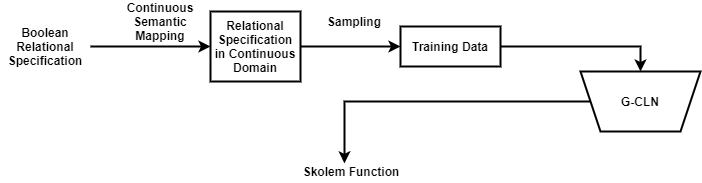
\includegraphics[scale=0.5]{workflow_bfs.png}
    \caption{Workflow}
    \label{fig:workflow}
\end{figure*}

% -------------- CODE FOR GOAL ARCHITECTURE ------------------
\subsection{Sampling Strategy}\label{sample}
Figure \ref{fig:sampling} describes the sampling pipeline that we have implemented to 
generate the training data.

\noindent\textbf{Random Sampling Strategy \Romannum{1}: }\label{sample1} In this we sample uniformly at random 
for input and output variables in the range $[0, 1]$. 
These random samples are then supplied to the continous mapping of relational specification (F). 
Output of F is then thresholded to get binary values. The ones that make F = 1 are taken to be 
positive samples. 

\noindent\textbf{Random Sampling Strategy \Romannum{2}: }\label{sample2} In this we collect positive samples 
as explained above and then add equal number of negative samples (F = 0) as well in the dataset.

\begin{figure*}
	\centering
    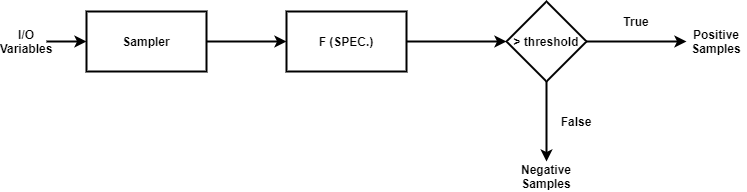
\includegraphics[scale=0.5]{sampling_bfs.png}
    \caption{Sampling Pipeline}
    \label{fig:sampling}
\end{figure*}

\noindent\textbf{Correlated Sampling: }\label{sample3} 
In this strategy, we first sample the input variables. Output variables are conditioned on input variables. 
This may help to capture the correlation betweenn input and output variables. we keep both positive and 
negative samples.

\noindent\textbf{Bias Sampling (Manthan): }\label{sample4}
Takes $F(X, Y)$ as input and returns a subset of satisfying assignments of $F$. Once these samples are generated 
we add noise to the data with range 0 to 0.2 and 0.8 to 1, to generate fractional sampling for training.

Table \ref{tab:tnorms} shows an example of random sampling.

\begin{table}[t]
\centering
\begin{tabular}{cccc}
	x: & y: & XOR(x, y) (thresholded value)\\ 
	0.9 & 0.2 & 1\\  
	0.85 & 0.01 & 1\\
    0.3 & 0.4 & 0
\end{tabular}
\caption{Example Samples for XOR(x, y) with threshold = 0.7 and Product t-norm}
\label{tab:tnorms}
\end{table}


\subsection{GCLN Architecture}\label{gcln}
Figure \ref{fig:gcln} shows the generic architecture that we use for predicting the skolem function from relational specifications.
It consists of 3 layers viz. Input Layer, Disjunction Layer, and Conjunction Layer. After each layer Gates are applied except for the final Conjunction Layer.
These Gates are the trainable weights of the neural network. More details below:

\smallskip
\noindent\textbf{Input Layer:} This layer is of shape 2N x 1, where N is the number of input variables in the given specification. 
Along with positive variables, we also consider their negations and include them in the input vector. For e.g. if the input variables 
are i1 and i2 then the input vector would contain $[i1, i2, \neg{i1}, \neg{i2}]$.

\smallskip
\noindent\textbf{Gates G1:} G1 is of shape 2N x K (K = No. of clauses and 2N = Size of each clause).
These Gates decides which input variables to be selected in each clause.

\smallskip
\noindent\textbf{Disjunction Layer:} This layer takes gated input variables. Shape of this layer is K x 1, where K is the maximum 
number of clauses that could possibly be present in the final solution. K is a hyperparameter and can be tuned.
%This layer decides which input variables to selected for each clause.

\smallskip
\noindent\textbf{Gates G2:} G2 is of shape K x M, where M is the number of output variables. 
It selects the clauses for the skolem function.

\smallskip
\noindent\textbf{Conjunction Layer:} This layer takes input the gated output of the Disjunction Layer. It is of shape 1 x 1. 
%This layer decides which clauses to be selected.

\begin{figure}
	\centering
    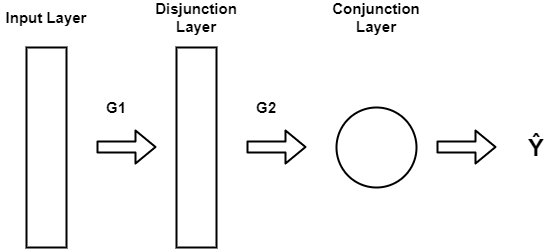
\includegraphics[scale=0.4]{gcln.png}
    \caption{GCLN Architecture}
    \label{fig:gcln}
\end{figure}

Due to the design of the network, the formula that we extract is in CNF form.
\newline

\noindent\textbf{Running Example:} Figure \ref{fig:ex} shows a running example of XOR(i1, i2, i3), 
where i1 and i2 are input variable and i3 is the output variable.

\begin{figure*}
	\centering
    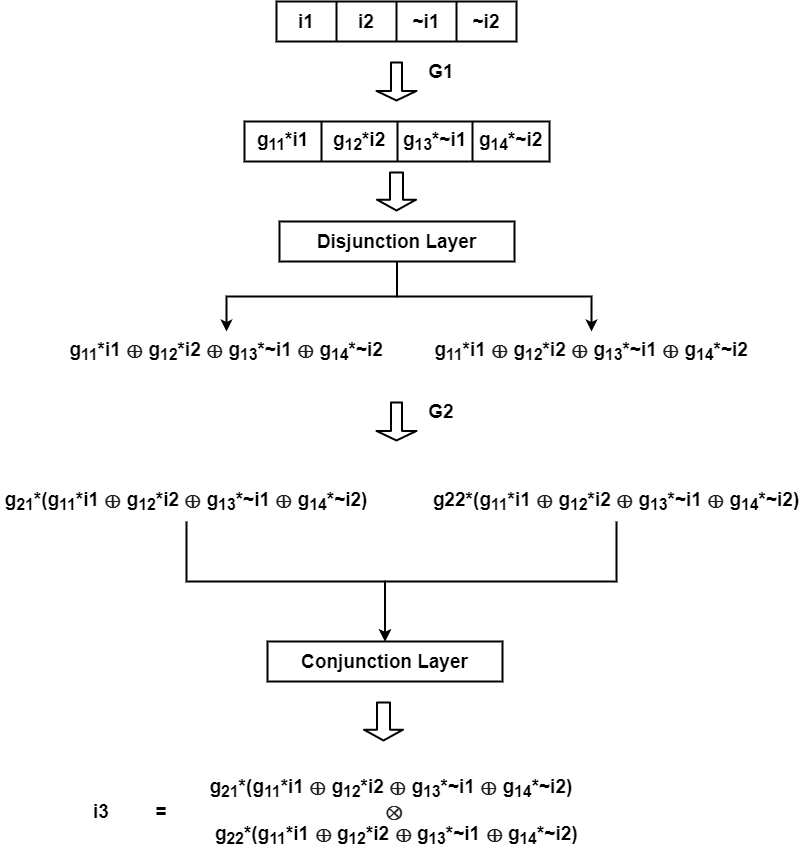
\includegraphics[scale=0.3]{example.png}
    \caption{Example run of GCLN over specification XOR(i1, i2, i3). Input Variable = i1, i2 and Output Variable = i3}
    \label{fig:ex}
\end{figure*}
% Figure \ref{fig:goal} describes the high level idea for synthesizing sketches from logical embeddings. We first sample a finite set of I/O examples from the logical specification. We wish to have a pre trained neural network for a given DSL that is trained to generate the required sketches when a logical specification and I/O specification are given as input. As a novel extension, it may also be possible for the NN to take as input a bad sketch and make decisions accordingly. This would be something similar to CEGIS(T) but using an NN. We then feed it to a traditional solver that solves the sketch using enumerative techniques if the sketch has non constant holes and constraint based techniques, if the sketch has constant holes. If the sketch is infeasible, then we use this to direct our NN to synthesize a better sketch. The meaning of an infeasible sketch is that there does not exist a valid (w.r.t. the DSL) completion of the sketch for the given specification.

% The major research question here is how to make the NN understand whether a given sketch is an infeasible sketch or not.

%---------- Proposed NN architecture-------
\section{Proposed Solution}
The problem of Boolean Function Synthesis can be posed as a learning problem. 
In an abstract sense, Observations O corresponds to boolean relational formula 
that serves as the specification for synthesizing skolem function.

let, F = Relational Specification (Observations)

\tab $\psi$ = Skolem Function Vector (Target)

And the aim is to learn a hypothesis function $'h'$ 

s.t.  $h(F;\hat{\theta}) = \hat{\psi}(X)$, where $\theta$ are learneable parameters of the model and
X denotes the set of input variables from the observations.

For a given dataset $\mathcal{D} = {(f_i, \psi_i)|1 \leq i \leq N}$, we want to minimize the 
expected loss between $\hat{\psi}(X) and \psi$

$$\text{Expected Loss: } E(l(\hat{\psi}(X), \psi)) \approx \frac{1}{N} \sum_{i=1}^{N} l(\hat{f_i}, \psi_i) $$

$$\hat{\theta} = \underset{\theta}{argmin} \frac{1}{N} \sum_{i=1}^{N} l(\hat{\psi_i}, \psi_i)$$

We model h using GCLN \ref{gcln}. 
The parameters in this network are the Gates ($\theta = (G_1, G_2)$) which acts like a switch 
for the input variables ($G_{1}$) or clauses ($G_{2}$).

As $\psi$ is not known to us, training a neural net over (F, $\psi$) is not possible. Therefore,
we perform sampling over
the boolean variables in formula F and mark the set of input variables (X) as the features and 
the set of output variables 
(Y) as the ground truth labels. Sampling strategies are discussed in detail in section \ref{sample}.

Sampling is done such that it captures the relation between X and Y. We exploit this fact and learn 
a function mapping $\psi$: X \rightarrow Y, wihch is our end goal.

We have implemented 4 different algorithms for solving this problem. We discuss these in the next section
\ref{algo} .

% If m is the number of input variables then 2*m is the size of each clause.



\section{Problem Formulations}\label{algo}
As of now we have come up with 4 different formulations for training the network. 
In this section we discuss those formulations. 
We also discuss their performance over a small set of toy examples.

\subsection{Regression}
This uses Random Sampling Strategy \Romannum{1}. Training data contains only positive samples. 
Output variables (Y) of the specification are the target variables while the input variables (X) are the features.
As the target values are real, most intuitive thing is to do regression.
The GCLN model regresses over the output variable. Loss function used here is mean square error loss.

Figure \ref{fig:regr} pictorially describes the algorithm.


\noindent\textbf{Intuitive Explanation for its Working: } With the given set up, model learns to predict Y's given X's.
That is it learn a function mapping from X to Y and this is the definition of the desired function to be synthesize. 
Now because we had sampled only samples which made the specification True, the function learnt for Y will output only 
those truth values of Y which would make the specification True.

\begin{figure}
	\centering
    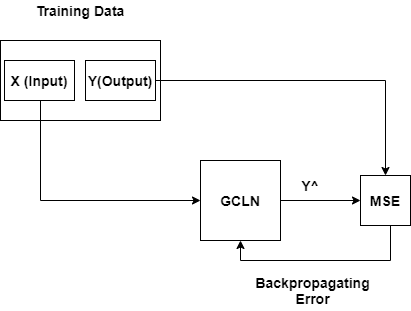
\includegraphics[scale=0.4]{regression.png}
    \caption{Regression Formulation}
    \label{fig:regr}
\end{figure}

\subsection{Classification Problem - 1}
Using Random Sampling Strategy \Romannum{1} we sample the training data.
In this case, the sampled real valued output variables (Y) are converted to binary ($Y_{bin}$) based on given threshold. 
Now we can consider $Y_{bin}$ as the class labels and learn a classifer over them. 
Loss function used in this case is Binary Cross Entropy Loss.

Figure \ref{fig:class1} describes it pictorially.

\noindent\textbf{Intuitive Explanation for its Working: } If the model learns a best fit
separating hyperplane, it will predict class labels $Y_{bin}$ for X. Which essentially means that the classifier is 
a mapping from X to $Y_{bin}$. As the data consists of only positive examples, the classifier would 
represent the required function.

\begin{figure}
	\centering
    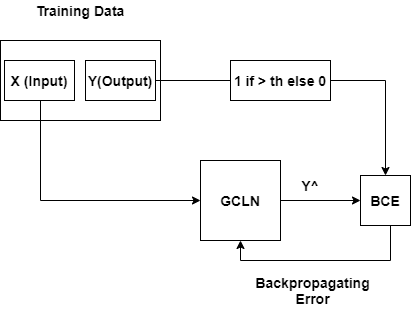
\includegraphics[scale=0.4]{class1.png}
    \caption{Classification - 1}
    \label{fig:class1}
\end{figure}

\subsection{Classification Problem - 2}\label{class2}
We use Random Sampling Strategy \Romannum{2}. Training data is $(X, F_{out})$ pairs, where, $F_{out}$ is the
output of F for the sampled input variables (X) and output variables (Y). i.e. X is features and $F_{out}$ 
are the class labels. Once $F_{out}$ is computed, Y is discarded.
While training we take the output of GCLN model $\hat{Y}$ and the input variables $X$ from trainig data
 and compute the value of $\hat{F_{out}}$ over them. In this set up, $\hat{Y}$ is the latent variable that 
 the model learns to predict. Loss function used is Binary Cross Entropy Loss over $\hat{F_{out}}$ and $F_{out}$
Figure \ref{fig:class2} descibes this pictorially.

\begin{figure}
	\centering
    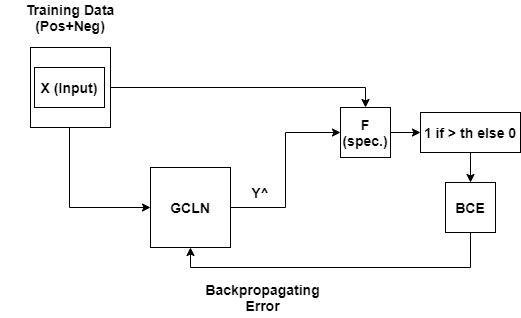
\includegraphics[scale=0.4]{class2.png}
    \caption{Classification - 2}
    \label{fig:class2}
\end{figure}

\noindent\textbf{Intuitive Explanation for its Working: } Here the model learns to predict correct $F_{out}$.
For that it first learns the latent variable $Y$ given only $X$ as its input. So, the model would learn a classifier
that tells which $Y$ to output such that it correctly classifies the $F_{out}$. It means that model will act as a 
mapping from X to Y such that it matches $F_{out}$ and $\hat{F_{out}}$. As the output of classifier mimics Y
for given X, it should represent the required skolem function.

\subsection{Classification Problem - 3}
This is same as \ref{class2} except the sampling strategy used here is correlated sampling
explained in \ref{sample3}.

\section{Results}
The output variable in the specification is replaced with the extracted formula from the network and checked for validity using z3Py Solver.
Figure \ref{fig:results} shows the preliminary results over 5 toy problems. The results are not very impressive at the moment but the hope 
is with intelligent sampling and better training procedure, this can be improved.

\begin{figure*}
	\centering
    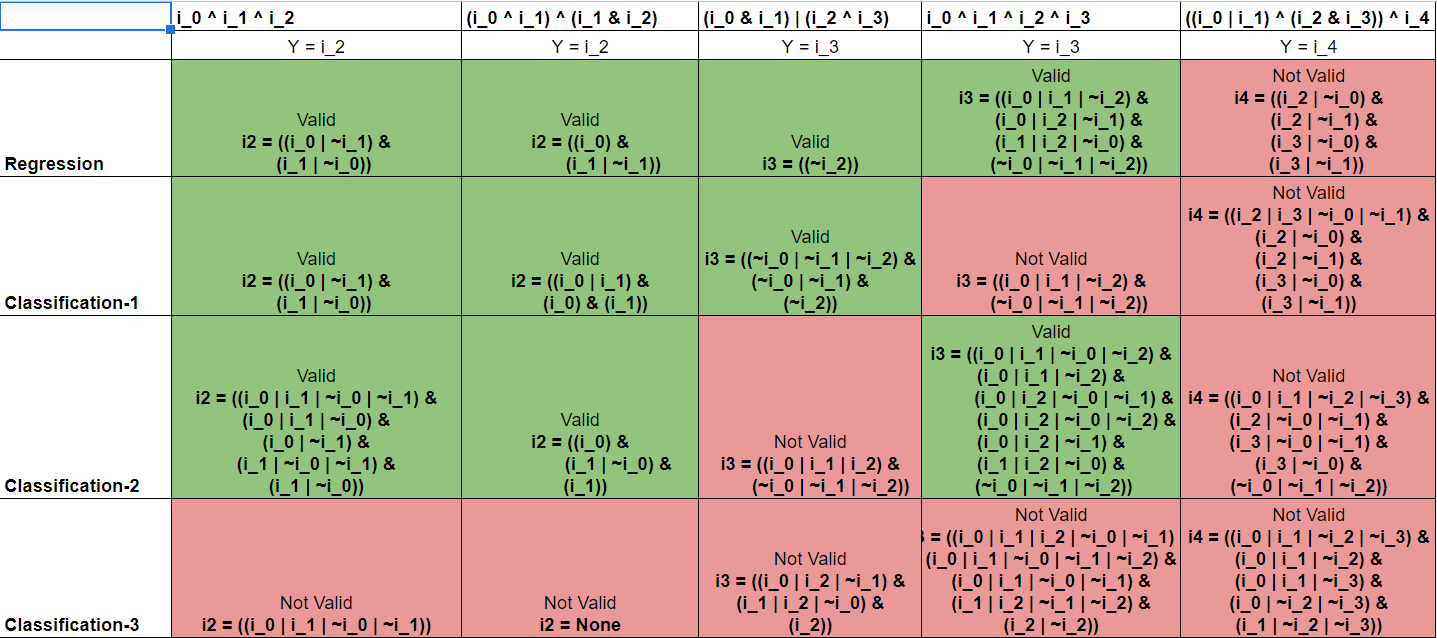
\includegraphics[scale=0.5]{results.png}
    \caption{Results on 5 toy Problems}
    \label{fig:results}
\end{figure*}
% \subsection{Generating training data}
Our aim is not to replace IO with generalized specifications but to aid these specifications with I/O examples.
Generating training data has been the bottleneck for this research work since it is not a trivial pursuit in our case.
Consequently, if we manage to generate synthetic SyGuS training data, it can prove to be a substantial contribution for Deep Learning based SyGuS research. Thus, generating data is one of the ideas we will focus on in this report. 
As discussed in Section \ref{dgnn}, DeepSynth's Neural Network architecture requires training data which is a pair of finite I/O specification and correct program. They achieve this by first randomly generating programs and inputs with certain restrictions.  Next, they generate the outputs by feeding these inputs to the generated programs. Thus, it is relatively easier to generate programs this way. Moreover, they claim to have promising results using this strategy.
This is encouraging for us to try a similar strategy for the generation of synthetic sygus benchmarks as well. However, we need training examples of the form (logical constraint + IO examples, correct program). The only option is to generate programs by feeding the constraints to different solvers. A natural question to ask would be how to generate millions of constraints? This is a challenging problem and will require a new data generation pipeline. We will discuss some ideas for data generation in this section.
Our aim is to train the Neural Network with constraint-program pairs in such a way that the NN can generalize well. Thus, it is important that we feed various combinations of the existing constraints to the NN.

\smallskip
\noindent\textbf{Mutations of existing SyGuS benchmarks:}
We can exploit properties of logical formulae such as commutativity, associativity etc to synthesize semantically equivalent but syntactically different constraints. For example, the formula A and B can be represented as B and A. Such mutations to existing formula will help in generation of constraints. Moreover, it should generate the same program which will aid the training of the NN.

\smallskip
\noindent\textbf{Using different solvers:}
The other possibility is to use different solvers so that they generate different programs for the same constraint. We have made this observation while experimenting with different tools. Correctness of these programs is important as well and hence a reliable solver such as CVC4 is important. As per our experiments, some solvers such as DryadSynth were not sound.

\smallskip
\noindent\textbf{Bounding synthesis time:}
Assume we require 80 million training examples as per DeepSynth. In such a case, we need 80 million constraints randomly generated using an intelligent strategy. Assuming we have access to a standard solver that can solve each constraint in approx 10 ms (which is a realistic expectation), the solving should take approx 10 days on a basic machine whereas increasing it to 50 ms may need 52 days of solving and 1 sec bound leads to 2.5 years of solving. Thus, bounding the synthesis time for constraints is important. More importantly, it is important to generate constraints that will be solvable within these bounds.

\smallskip
\noindent\textbf{Random generation of constraints:}
The previous ideas may not scale to millions of training data that we need. Thus, at some point, we have to look into generating random constraints using ideas from DeepSynth as a starting point. This becomes challenging in our situtation as the structure of the constraints change for different classes of SyGuS benchmarks. For example, Loop Invariant SyGuS benchmarks have a PRE, TRANS, POST format whereas the others do not. Thus, it is prudent to decide a class of benchamarks first and proceed.

\smallskip
\noindent\textbf{Number of training examples:}
Since we are using logical constraint and I/O specification as an input to the NN instead of just I/O specifications, it may be possible that we require fewer examples for training. However, this can only be empirically evaluated.


%---------- SyGuS Sketcher: A preliminary prototype-------
% \section{SyGuS-Sketcher: A preliminary prototype}

Instead of solving the larger problem as mentioned in the previous section, we decided to solve a sub-problem first.
We have begun implementing a preliminary prototype as a tool which we call SyGuS-Sketcher. SyGuS-Sketcher is built atop DeepSynth \cite{polgreen2020counterexample} and is available on github.\footnote{\url{https://github.com/stanlysamuel/sygus-sketcher}}. In this section, we discuss the tool architecture for SyGuS-Sketcher  and experimentation direction. The aim of this prototype is to show that sketches for logical specifications can indeed help improve the performance and number of benchmarks solved as compared to DeepSynth. This is our hypothesis.

\subsection{Tool architecture}

Figure~\ref{fig:curr} shows the prototype architecture. As you can see, the architecture is similar to DeepSynth except for two modifications. First, out of the top K candidates selected by the DeepSynth's NN, we select the candidate most likely to be correct, which is a complete program. Next, we replace the constant values with constant literals to generate a sketch. This is as good as assuming that we do not trust the constants generated by the Neural Network but use existing sketch compilers to fill up the program while guaranteeing the correctness of the specification. Thus, this boils down to a problem of solving sketches with constant holes which is exactly what the Sketch tool\cite{10.5555/1714168} does. However, for the bit-vector invariant generation benchmarks that we use, Sketch has limited support. For example, bit-vector subtraction and relational operators are not supported in Sketch due to which we had to look for other options. Thus, we looked into CEGIS(T) verifier which has this support. They have a Fourier Motzkin and an SMT based verifier and we need to decide which one fits in our case. We are currently in the process of implementing this integration. This is the second modification from DeepSynth.

%\Stanly{Try explaining the sketches with an example}


% ---------------------- CODE FOR OUR CURRENT IMPLEMENTATION --------------------------
\begin{figure*}
\resizebox{!}{!}{%
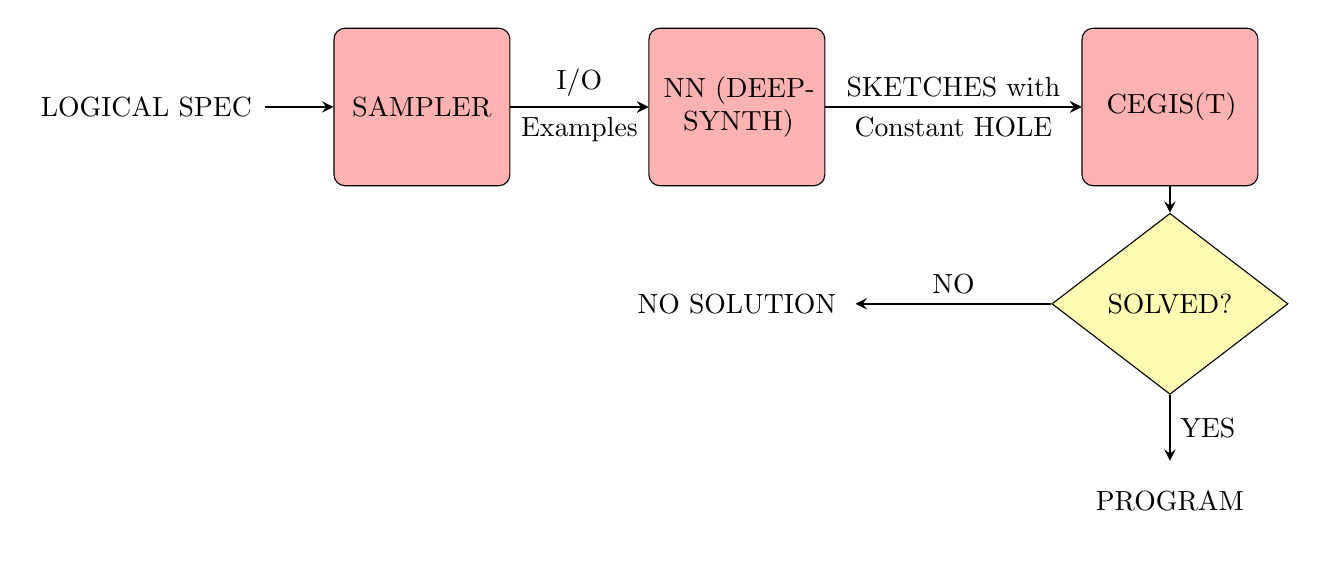
\begin{tikzpicture}[node distance=2cm]
\node (pr) [process] {LOGICAL SPEC};
\node (sam) [startstop, right of=pr, xshift=1.5cm] {SAMPLER};
\node (nn) [startstop, right of=sam, xshift=2cm] {NN (DEEPSYNTH)};
\node (sol) [startstop, right of=nn, xshift=3.5cm] {CEGIS(T)};
\node (bs) [process, below of=nn, yshift=-0.5cm] {NO SOLUTION};
\node (dec1) [decision, below of=sol, yshift=-0.5cm] {SOLVED?};
\node (sn) [solution, below of=dec1, yshift=-0.5cm] {PROGRAM};
\draw [arrow] (pr) -- node[anchor=south] {} (sam);
\draw [arrow] (sam) -- node[anchor=south] {I/O} (nn);
\draw [arrow] (sam) -- node[anchor=north] {Examples} (nn);
\draw [arrow] (nn) -- node[anchor=south] {SKETCHES with} (sol);
\draw [arrow] (nn) -- node[anchor=north] {Constant HOLE} (sol);
\draw [arrow] (sol) -- node[anchor=south] {} (dec1);
\draw [arrow] (dec1) -- node[anchor=south] {NO} (bs);
\draw [arrow] (dec1) -- node[anchor=west] {YES} (sn);
\end{tikzpicture}
}
\caption{SyGuS-Sketcher architecture}
\label{fig:curr}
\end{figure*}

\subsection{Planned experiment}

We plan to test this prototype against DeepSynth's 88 bit-vector invariant benchmarks. We describe a subset of these benchmark timings below: \\

\begin{tabular}{ |p{2cm}||p{2cm}|p{2cm}|  }

 \hline
 Benchmarks & DeepSynth  & SyGuS-Sketcher\\
 \hline
 anfp-new   &  23.7529s & .   \\
 formula22    & 44.5536s & . \\
 hola.05 &   165.086s & .  \\
array-new & 76.1318s  & . \\
 cegar2-new&106.402s  & .\\
 \hline
\end{tabular} \\

As you can observe, DeepSynth takes a considerable amount of time whereas traditional solvers without neural network architectures have an order in milliseconds. This is where we expect Sketches to play a role in improving the performance time.



 
%---------- Future work -------
\section{Future Directions}
\noindent Following is a consolidation of the discussions held in previous meetings.

\subsection{Sampling Strategy}
\noindent\textbf{Seed based Sampling:}
Instead of going for Random Sampling, we can use a few seed examples from the SAT solver. 
Once we have the seed examples, we can sample around these examples to get the training data.
This would give more accurate training data faster.

\smallskip
\noindent\textbf{Simulated Annealing:} 
This is another way to avoid Random Sampling. Simulated Annealing would be faster and 
won't require the seed examples as well. This method is based on Energy Functions.

\subsection{Training}
\noindent\textbf{Counter Example Guided Training:} If the first output of the model doesn't give us the 
intended result, we can generate countere examples using a SAT solver and feed that back to the Network
 through a feedback loop. This will tell exactly where the model is failing.

 \smallskip
 \noindent\textbf{Loss Function:} Instead of computing the loss over model's numerical output, 
 can we compute loss over final formula extracted from the network? 

 \noindent As we don't have final formulae in our dataset, this idea doesn't seem to work as of now.

 \smallskip
\noindent\textbf{Hyperparameter Search:} Instead of trying out different hyperparameter values manually, 
we can automate this process. An efficient way to do this is through Hyperparameter Search.

%---------- Conclusion ----------
% % !Tex root=main.tex

\section{Conclusion}

In this report, we have proposed a research idea and a plausible line of attack. We have also started preliminary work in implementing the prototype and experimental evaluation is under way. 
%We also discussed interesting research threads in the future work section

%Our approach combines 
%In future work,
%
%This work lays the foundation for some interesting extensions.
This report highlights the following contributions: 1) A line of direction to generate synthetic dataset for SyGuS benchmarks, 2) A "concolic" neural network architecture using logical embeddings and I/O embeddings and 3) A prototype tool SyGuS-Sketcher using existing techniques with experimentation plan.

%---------- Bibliography ----------
% \bibliographystyle{splncs04}
\newpage
\bibliography{bib}
\bibliographystyle{abbrv}

%---------- Appendix: Stanly ----------
\clearpage
\section{Network architecture to represent CNF formulae}

In this section,  we design three architectures for the boolean function synthesis problem. Each of these architectures are used to learn formulae in conjunctive normal form (CNF).  The training phase is guided using an oracle that provides counterexamples to the formulae synthesized using the network.  In our setting, the oracle is a verifier for the boolean function synthesis problem.  In this problem,  for a given function, there could be multiple solutions possible and hence multiple local minima.  The choice of minima depends on the counterexamples generated by the counterexample loop.

\subsection{Architecture 1: Single output GCLN}

Let the CNF formula be $F$ as shown below:

\[ F = \bigwedge_{j = 1}^m \ (\  \bigvee_{i=1}^{2n}\  (x_i\ .\ g_{ij})\ .\ g_j)\]

where,  \\ 
$n$ = number of input variables (i.e.,  $|V|$), \\
$m$ = number of clauses and is bounded by $2^{2n}$ \\
$x_i$ = set of variables and their negations (i.e.,  $2|V|$), .\\
$g_{ij}$ = 1 iff the $i^{th}$ variable is used in the $j^{th}$ clause.\\
$g_{j}$ = 1 iff the $j^{th}$ clause is used for the output.\\

The GCLN architecture for $m = 3$ and $V = \{ x\}$ is as follows: \\

Enter diagram here \\

The network has three layers where the middle (disjunct) layer is variable in size.

Although this network has a single output,  we may be able to synthesize functions for multiple outputs by:\\
(a) sampling intelligently,  \\
(b)using a dependency guided loop after every function synthesized (not sure how as we do not know how to extract a single correct function separately)



\subsection{Architecture 2: Multiple output GCLN with a shared layer}

\subsection{Architecture 3: Multiple output GCLN without a shared layer}

\section{Network architecture to represent DNF formulae}

The architectures used to synthesize CNF formulae can also be used to learn formulae in disjunctive normal form (DNF).  In such a case, the middle layer would now consist of T-conorms instead of T-norms.

\section{Possible advantages of our approach over Manthan}
\begin{itemize}
\item Manthan is constrained to use DNF formulae only whereas we can use both CNF and DNF as the size of the formula is within our reach.  $SAT \leq_P 3-SAT$ tells us that for any formula there exists an equisatisfiable formula in CNF of polynomial size.  No  such result is known for DNF.  All such reductions give an exponentially sized DNF formulae. Can we somehow expect, using this information, that we can generate smaller formulae?

\end{itemize}

%---------- Appendix: Synthesizing sketches using RL ----------
%\clearpage
%\documentclass{article}
\section{Learning Program Sketches from SMT Specification
using Reinforcement Learning}
% if you need to pass options to natbib, use, e.g.:
%     \PassOptionsToPackage{numbers, compress}{natbib}
% before loading neurips_2020

% ready for submission
% \usepackage{neurips_2020}

% to compile a preprint version, e.g., for submission to arXiv, add add the
% [preprint] option:
%     \usepackage[preprint]{neurips_2020}

% to compile a camera-ready version, add the [final] option, e.g.:
%     \usepackage[final]{neurips_2020}

% to avoid loading the natbib package, add option nonatbib:

% The \author macro works with any number of authors. There are two commands
% used to separate the names and addresses of multiple authors: \And and \AND.
%
% Using \And between authors leaves it to LaTeX to determine where to break the
% lines. Using \AND forces a line break at that point. So, if LaTeX puts 3 of 4
% authors names on the first line, and the last on the second line, try using
% \AND instead of \And before the third author name.

\begin{abstract}
  This work aims at performing a literature review around Program Synthesis using Machine Learning techniques and exclusively writing reviews for the tools like SKETCHADAPT and META-SOLVER. It also formulates a problem for synthesizing sketches for the General Track of SyGuS benchmarks and proposes a novel model META-SKETCHER aiming to solve it. 
\end{abstract}

\subsection{Introduction}

Program Synthesis is an age-old problem of generating programs automatically that satisfies the user intent called Specification. It basically consists of three components: 1) Specification, 2) DSL, and 3) Search. Many recent advances in this field is due to the fusion of Machine Learning tactics with it. Here, I briefly review some most important literature that gives a basic understanding of the current state-of-the-art.

\subsubsection{Literature Review}
\paragraph{Deductive Synthesis :}
Some initial works on automatic program generation were based on Automated Theorem Provers [1, 2, 3]. The key idea followed by them was to construct the proof of the logical specification given by the user and then extract the logical program using it. Such approaches required the user to specify complete logical specs which are often as complex as writing the programs itself. Also, it proved to be intractable due to huge program space. Syntax Guided Synthesis (SyGuS) [4] restricts the program space by defining a Domain Specific Language (DSL) with the help of a Grammar. \ref{problem} states the formal SyGuS problem statement.

\paragraph{Inductive Program Synthesis (IPS) :}
Inductive Program Synthesis (IPS) is based on inductive specifications (for e.g. I/O Examples, Demonstrations, Natural Language, or Partial Programs) emerged as an alternative. FlashMeta [5] by Polozov and Gulwani transforms the relationships between I/O pairs to intended programs. Along with syntactic specification it also includes the semantics of the language and follows a Divide and Conquer strategy to get the final program in real time. FlashFill [6] is a successful application of FlashMeta architecture used by Microsoft in spreadsheets. Program Synthesis by Sketching [7] by Armando Solar-Lezama synthesizes programs from partially complete programs called SKETCH. 

\paragraph{Program Synthesis using Machine Learning :}
Menon et al. [8] uses the I/O examples to learn the probability distributions over productions in the Grammar converting it to Probabilistic CFG. This gives an order of the magnitude better performance over an enumerative baseline.  The PCFG approach fails to include the contextual information stored in the partial programs generated at each instant while searching in the program space. 

\paragraph{Neural Program Synthesis (NPS) :}
RobustFill by Devlin et al. [9] and DeepCoder by Balog et al. [10] are some recent advance in NPS. RobustFill designs a Neural Network that replaces the entire enumerative search part which is then trained to output a complete program. This may not guarantee the correctness of the final programs. Whereas DeepCoder uses a Neural Network to prune the search space rather than replacing the search part entirely.
This work proposes a novel approach for synthesizing programs from \textbf{logical spec.} with the help of \textbf{intermediate sketches}. As logical specs. can cover all possible program behavior and I/O specs. fails guarantee completeness. For ex. Given f(x) = 2*x, one can understand that the program output is twice the input, it cannot be derived correctly from I/O pair (1,2). It may get confused between addition of 1 and multiplication by 2. Therefore, this work primarily aims at solving SyGuS problems that appear in \href{https://sygus.org/}{SyGuS Competition}. Following two papers forms the basis of the work.

\subsubsection{Review: Learning to Infer Program Sketches (SKETCHADAPT)}
The key idea here is to generate program sketches from user spec. (I/O, natural language) that flexibily manages the work load between Neural Synthesis and Symbolic Search. \textbf{Sketches} are valid program tree in the DSL, where any number of sub-trees has been replaced by a special token called <HOLE>. Intuitively, this token designates locations in the program tree for which pattern-based recognition is difficult, and more explicit search methods are necessary. SKETCHADAPT [11] can be divided into two components: 1) \textbf{Neural Sketch Generator} which is a Seq2Seq neural architecture. It takes the spec. as input sequence and produces a good sketch as a sequence of tokens, and 2) Program Synthesizer which takes the generated sketch and outputs a final program by choosing grammar productions based on learned production probabilities. Generating a good sketch prunes out a large part of program space, thereby improving the synthesis time. Due to use of a symbolic search to fill up the sketches, programs produced are more generic. While this work is a huge success for the domains of List Processing and String Processing, it does not work at all on the kinds of problems found in the SyGuS-Comp where user intent is in the form of Satisfiability Modulo Theory (SMT) formulae. Further, it requires millions of training data for training the network which is not readily available for domains as in SyGuS.

\subsubsection{Review: Learning a Meta Solver for Syntax-Guided Program Synthesis}
Both the logical (semantic) spec and the grammar (syntactic spec) have complex structures and can vary from task to task, posing significant challenges for learning across different tasks. Moreover, supervision is often unavailable for domain-specific synthesis tasks. Therefore, it's natural to formulate the problem in a Reinforcement Learning (RL) framework where the Environment is the Program Space specified by Grammar, Meta-Solver is the agent that performs an action by selecting a grammar production based on the reward returned by a SAT/SMT solver. The Meta-Solver [12] consists of three components: 1) an encoder, which embeds both the logical specification and grammar at the same time using a GGNN \footnote{Gated Graph Neural Network}; 2) a grammar adaptive policy network which enables learning a transferable policy; and 3) a RL algorithm that jointly trains the embedding and adaptive policy with sparse reward \footnote{Rewards are called sparse when it is available only when the goal is reached (in this case a program is found)}. Comparing an Out-Of-Box setting which is trained and tested over same data with the two state-of-the-art classical synthesis tools CVC4 and EUSOLVER, it solves 129 and 153 out of 214 circuit synthesis problems respectively. While the Meta-Solver achieves speedup ranging from 2x up to 100x. Even though it performs really well in comparison to other state-of-the-art solvers such as CVC4 and EUSOLVER, the problem domain is too restrictive as it only solves the problems in Cryptographic circuit synthesis SyGuS benchmarks [13]. Also it does not considers generating sketches and combining a symbolic approach to complete it instead of fully dending upon RL.
%Sections \ref{gen_inst}, \ref{headings}, and \ref{others} below.

\subsection{Problem Formulation}
\label{problem}
The Syntax-Guided Synthesis (SyGuS) problem is to synthesize a function f that satisfies two kinds of constraints:
\begin{itemize}
    \item a syntactic constraint specified by a context-free grammar (CFG) G, and
    \item a semantic constraint specified by an SMT formula $\phi$ built from symbols in a background theory T along with f
\end{itemize}
This work aims at extending the work of [Meta-Solver] and generalizing it for SyGuS problems other than Cryptographic circuit synthesis problems by using the idea of sketches from the [SKETCHADAPT] paper.

Given a Dataset of N tasks $D = \{(\phi_i, G_i)\}_{i=1}^{N}$, I propose the following components for the proposed tool.

\begin{itemize}
    \item Using Gated Graph Neural Network for learning the representation for the specification $\phi$ and the grammar G so that the synthesis process can utilize the structural information present in logical specification and grammar
    \item Learning a Policy $\pi_{\theta} : (\phi, G) \rightarrow \sigma$ where $\theta$ is the parameter of the learned policy and $\sigma$ is the sketch or the partial program.
    \item Learning production probabilities p for the grammar productions i.e. for each non terminal $\alpha$, probabilities should be assigned to each of it's expansion $ \alpha \rightarrow \beta_{i} $
    \item A Solver for solving sketches to get the final program using Symbolic Searches such as  enumerative search guided by the production probabilities.
\end{itemize}

Two prime difficulties faced while solving such a problem are : 1) Scarcity of dataset: the dataset present in the SyGuS benchmarks are not enough to train a Neural Network, it requires millions of solved benchmarks, and 2) Sketches are not complete programs, so a SAT or an SMT solver cannot verify it and hence cannot return a reward to the policy learner. I address these issues in following section.

\subsection{META-SKETCHER}
\label{headings}

This section presents the META-SKETCHER model (see figure 4) that attempts to solve the three problems stated in section \ref{problem}

\begin{figure*}[!htp]
\label{metasketcher}
\centering
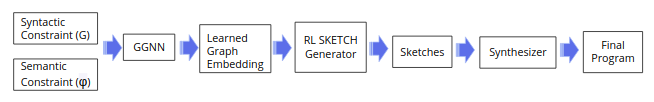
\includegraphics[width=\textwidth,height=2.0cm]{metasketcher.png}
\vspace*{-0.9cm}
\caption{META-SKETCHER Proposed Model}
\vspace{-1.2em}
\end{figure*}

\subsubsection{Formal Definitions}

Following are the formal definitions of some of the key terms.

\paragraph{Semantic Spec $\phi$ :}
These are formulas that consists of constraints written in the form of SMT formulae. It follows the same grammar G which is specified for the output program.

\paragraph{CFG G :}
A context free grammar (CFG) G is as defined in the [META-SOLVER] paper except the following modification.

The grammar should be modified for sketch generation by adding a new token <HOLE> which is used to replace any sub-tree in the program tree leaving that part to be searched using a symbolic search.

\paragraph{Output Sketch $\sigma$ :}
The Output Sketch $\sigma$ is a partial program generated using the grammar G. A good sketch will be the sketch that leads to final program f which satisfies both syntactic and semantic specifications.

\paragraph{Output Program f :}
The Output Program f is the final program that is generated from intermediate sketches. The final program f must satisy both syntactic (grammar G) and semantic (SMT formula $\phi$) specification 

\subsubsection{Novel Idea :}
Synthesizing sketches for General SyGuS benchmarks where the specifications are in the form of logical formulae instead of input output examples using a Reinforcement Learning framework. The policy network should learn to output partial programs based on the rewards.

\paragraph{Rewards :}
As sketches are incomplete programs it should not be verified by SAT/SMT solvers with the given semantic specification, one needs to consider some indirect ways of receiving rewards. Using the learned production probabilities, likelihood of the sketches could be calculated, and this can easily serve the purpose.


Both of these selected works does not talk about synthesizing programs for General SyGuS benchmarks. Also none has used sketches for it. As use of sketches in [SKETCHADAPT] has proved its applicability, I vouch for 

\subsection{Experiments}
\label{others}

\paragraph{Experimental Setup :}
Following experiments are done on Intel(R) Xeon(R) CPU E5-2420 v2 @ 2.20GHz with 32 GB Memory

\subsubsection{META-SOLVER}
I tested the META-SOLVER on 30 out of 214 SyGuS Cryptographic circuit synthesis benchmark problems. It elegantly solved 22/30 problems in an average time of $\sim0.32$ secs. While a state-of-the-art cvc4 ran out of memory for all the selected 30 problems. 

Because of less time, I could not perform a full fledged experiment as it requires more than 6 hours to conclude that a problem cannot be solved.\footnote{The SyGuS 2017 competition gives each solver 4-core 2.4GHz Intel processors with 128 GB memory and
wallclock time limit of 1 hour}

The excel sheet for the results can be found at \href{https://indianinstituteofscience-my.sharepoint.com/:x:/g/personal/raviraja_iisc_ac_in/EU-Um2g9igVJk5XrmXZoL1IBR_DlPHCtAWpxcVPZtu4n_Q?e=Krd9t5}{Excel Sheet for the Experments performed}

\subsubsection{Preliminary Results}
I did try to generate sketches using the existing framework of META-SOLVER but found that it is not able to handle infinite grammar (recursive grammar) and gives Recursion Error.

\subsection{Conclusion}
In this work I did a Literature Review for the field of Program Synthesis and it's improvements using Machine Learning. I exclusively reviewed the two recent tools for synthesizing programs one with sketches and other without sketches namely SKETCHADAPT and META-SOLVER respectively. The study shows that no work has been done around generating sketches for SyGuS problems where the specification is in the form of SMT formulae. The META-SKETCHER model presented in this work will be implemented in the near future.

\subsection*{References}
\small

[1] C. Cordell Green. Application of theorem proving to problem solving. In IJCAI, pages 219–240, 1969.

[2] Zohar Manna and Richard J. Waldinger. Toward automatic program
synthesis. Commun. ACM, 14(3):151–165, 1971.

[3] Richard J. Waldinger and Richard C. T. Lee. PROW: A step toward
automatic program writing. In IJCAI, pages 241–252, 1969.

[4] Rajeev Alur, Rastislav Bodík, Garvit Juniwal, Milo M. K. Martin,
Mukund Raghothaman, Sanjit A. Seshia, Rishabh Singh, Armando
Solar-Lezama, Emina Torlak, and Abhishek Udupa. Syntax-guided
synthesis. In Formal Methods in Computer-Aided Design, FMCAD,
pages 1–8, 2013.

[5] Oleksandr Polozov and Sumit Gulwani. FlashMeta: a framework for
inductive program synthesis. In Proceedings of the 2015 ACM SIGPLAN
International Conference on Object-Oriented Programming, Systems,
Languages, and Applications, OOPSLA 2015, pages 107–126, 2015.

[6] Sumit Gulwani. Automating string processing in spreadsheets using input-output examples. In Proceedings of the 38th ACM SIGPLANSIGACT Symposium on Principles of Programming Languages, POPL
2011, Austin, TX, USA, January 26-28, 2011, pages 317–330, 2011.

[7] Armando Solar-Lezama. Program synthesis by sketching. ProQuest,
2008.

[8] Aditya Krishna Menon, Omer Tamuz, Sumit Gulwani, Butler W. Lampson, and Adam Kalai. A machine learning framework for programming by example. In Proceedings of the 30th International Conference on Machine Learning, ICML 2013, Atlanta, GA, USA, 16-21 June 2013,
pages 187–195, 2013.

[9] Devlin, J., Uesato, J., Bhupatiraju, S., Singh, R., Mohamed,
A.-r., and Kohli, P. Robustfill: Neural program learning
under noisy i/o. arXiv preprint arXiv:1703.07469, 2017.

[10] Matej Balog, Alexander L. Gaunt, Marc Brockschmidt, Sebastian
Nowozin, and Daniel Tarlow. DeepCoder: Learning to write programs.
CoRR, abs/1611.01989, 2016.

[11] Maxwell I. Nye, Luke B. Hewitt, Joshua B. Tenenbaum, and Armando Solar-Lezama. Learning to
infer program sketches. In Kamalika Chaudhuri and Ruslan Salakhutdinov (eds.), Proceedings
of the 36th International Conference on Machine Learning, ICML 2019, 9-15 June 2019, Long
Beach, California, USA, volume 97 of Proceedings of Machine Learning Research, pp. 4861–4870.
PMLR, 2019.

[12] X. Si, Y. Yang, H. Dai, M. Naik, and L. Song, “Learning A Metasolver For Syntax-guided Program Synthesis,” ICLR, 2018.

[13] Hassan Eldib, Meng Wu, and Chao Wang. Synthesis of fault-attack countermeasures for cryptographic circuits. In Swarat Chaudhuri and Azadeh Farzan (eds.), Computer Aided Verification, 2016.

%Ravi



\end{document}
